
% compiler-structure.tex: generic organization of a compiler.

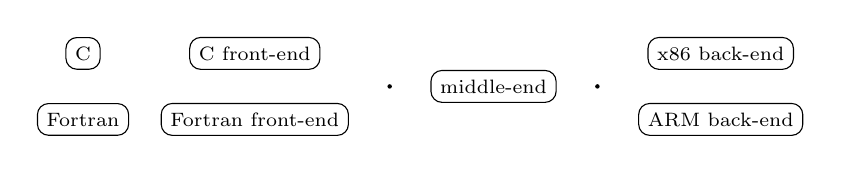
\begin{tikzpicture}
[
  every node/.style={
    font=\scriptsize
  },
  cell/.style={
    rectangle,
    rounded corners,
    draw
  },
  point/.style={
    circle,
    fill,
    inner sep=.2mm
  },
  tip/.style={
    ->,
    shorten >=.5mm,
    shorten <=.5mm
  },
  man-tip/.style={
    tip,
    to path={-| (\tikztotarget)}
  },
  rman-tip/.style={
    tip,
    to path={|- (\tikztotarget)}
  }
]

\matrix [column sep=4mm]
{
\node (c-language)   [cell] {C};             &
\node (c-front-end)  [cell] {C front-end};   &
\node ()             []     {};              &
\node ()             []     {};              &
\node ()             []     {};              &
\node (x86-back-end) [cell] {x86 back-end}; \\

\node ()               []      {};           &
\node ()               []      {};           &
\node (middle-end-in)  [point] {};           &
\node (middle-end)     [cell]  {middle-end}; &
\node (middle-end-out) [point] {};           &
\node ()               []      {};          \\

\node (fortran-language)  [cell] {Fortran};           &
\node (fortran-front-end) [cell] {Fortran front-end}; &
\node ()                  []     {};                  &
\node ()                  []     {};                  &
\node ()                  []     {};                  &
\node (arm-back-end)      [cell] {ARM back-end};     \\
};

{ [start chain]
\chainin (c-language)    [join];
\chainin (c-front-end)   [join=by tip];
\chainin (middle-end-in) [join=by man-tip];
}

{ [start chain]
\chainin (fortran-language)  [join];
\chainin (fortran-front-end) [join=by tip];
\chainin (middle-end-in)     [join=by man-tip];
}

{ [start chain]
\chainin (middle-end-in)  [join];
\chainin (middle-end)     [join=by tip];
\chainin (middle-end-out) [join=by tip];
}

{ [start chain]
\chainin (middle-end-out) [join];
\chainin (x86-back-end)   [join=by rman-tip];
}

{ [start chain]
\chainin (middle-end-out) [join];
\chainin (arm-back-end)   [join=by rman-tip];
}
\end{tikzpicture}
